\documentclass[a4paper,12pt]{article}

\usepackage{url, hyperref, graphicx}

\begin{document}

\title{Project 2}
\author{Chip Bell}
\date{March 31, 2015}
\maketitle

\section{Problem Description}
The Washington Metropolitan Area Transit Authority's Metrorail system in many respects is a driving factor in the
expansion of the city. With Washington's fixed size, reliable and cost-efficient transportation for metro area
residents is crucial for maintaining the city's economy. However, this is a difficult task in that there are many
variables involved, such as human error, mechanical failure, and even acts of nature.

Therefore for this project, I will be simulating the metrorail system using data collected from the WMATA API
\cite{wmataapi}, which provides realtime estimates of train arrival. Furthermore, I will simulate the impact that track
closures have on train throughput.

\section{Previous Work}
Many large cities have rapid transit systems, so considerable research time has been invested on building reliable
subways. Commercial software such as OpenTrack \cite{opentrack} have been developed, and even video games such as Train
Simulator \cite{trainsimulator} and Open Rails \cite{openrails}. Algorithms for handling single, double and tracks exist, such as the basic intuitive
algorithm for sharing tracks between trains presented by Fiorini and Botter \cite{fioroni}. Dessouky and Leachman
\cite{dessouky_leachman_95} provide an event-driven algorithm for single and double track rail networks, incorporating
acceleration. Lu et al \cite{quan_lu} expand the model to triple tracks while enhancing the acceleration model to
handle multiple track speed limits.

\section{Basic Architecture}
The nature of trains lends itself to a model that incorporates resource sharing. For instance, only a single train can
occupy a particular section of track at a given moment. Furthermore, if two trains are sharing a track, they cannot
be going in different directions unless they have already past each other, lest they collide. This issue is addressed
by Fioroni \cite{fioroni}.

A common occurrence in the metro system is that between two stations a particular section of track is under
maintenance, forcing trains going both directions to share a track. These basic issues result in a couple of clear
concepts that we'll incorporate in our model.

The first is a train. A train encapsulates all of the information relevant to our application: which line it is
(Orange, Blue, or Silver), it's direction, and it's location within the system. Measuring the throughput of trains
in the system will be our primary statistic when running the simulation.

The other important entity to be concerned with is the track itself. From a queueing standpoint, it is a limited
resource that only a single train can use at a single point. If a piece of track is occupied by a train, all other
trains must wait before they may proceed through the track (in an assumed FIFO order). It is for this reason that
most train systems do prefer to have a second track to prevent blocking for trains going in opposite directions.
So, in our case we can treat a section of track as a queue that can only process a single train at a time. Between
stations, there are generally two sections of track. However, track maintenance would cause a track to close, forcing
opposing tracks to share.

Because of this, we can represent the entire metro as queuing network with sections between stations as the queue. In
our case, we will only be modeling the section of track between Rosslyn and Stadium-Armory where the Orange, Blue, and
Silver share a track (See \ref{fig:metromap}). Since there are no track crossovers, we can consider these three lines
to be isolated from other lines.

\begin{figure}
\begin{center}
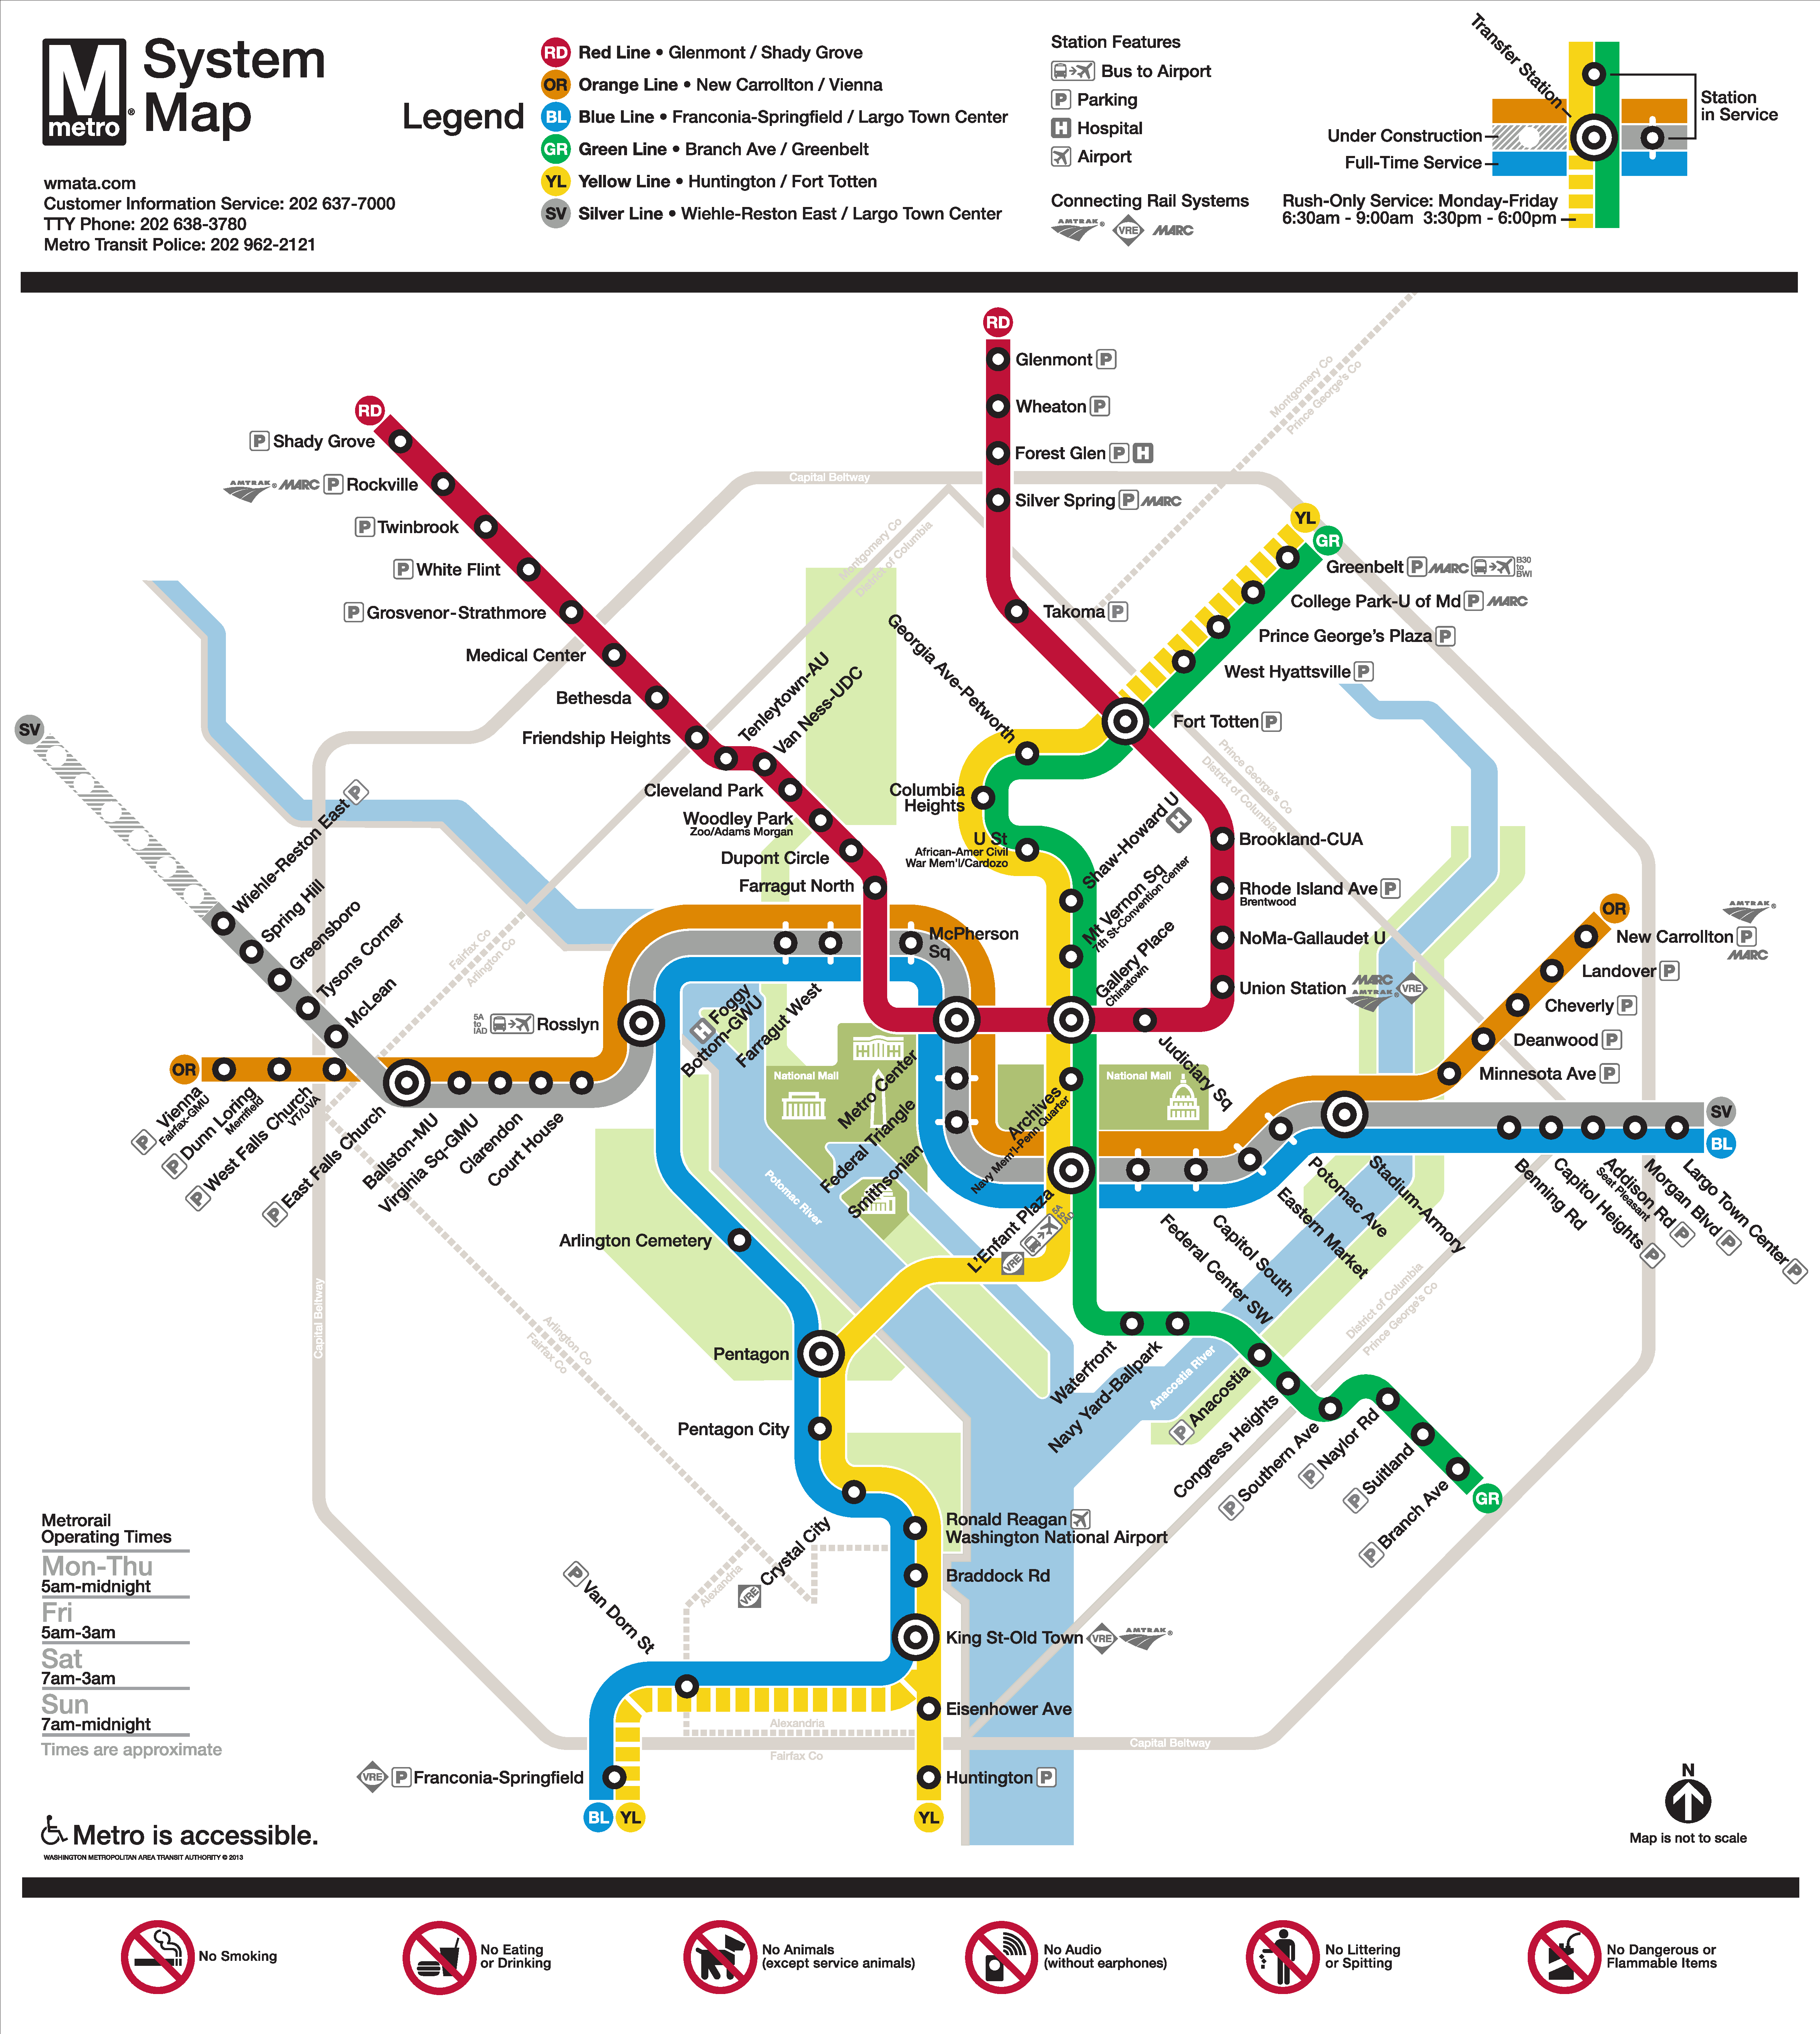
\includegraphics[width=5in]{../images/metro_map.pdf}
\caption{\small \sl WMATA Metrorail Map \label{fig:metromap} \cite{fioroni}}
\end{center}
\end{figure}

\section{Data Collection}

\subsection{Query Design}
Viewing this as a queueing problem, there are some ``missing pieces'' that our model did not incorporate, namely the
arrival rate of trains and the service time for a single train. Instead of attempting to calculate these based on 
numerical models of motion, we can instead use the WMATA API \cite{wmataapi} to calculate this.

The API provides data by station with an estimate at each station of the wait time until the next train. For instance,
the API for a station on the blue line might list a train to Franconia-Springfield (westbound) in 1 minute. If there
also happens to be an Orange that passes through that station, you may also see an estimate for the next Orange (if it
close enough).

Given this information, we can calculate how often a train runs simply by marking the timestamp of the API call and
offset by the estimated time until arrival provided by the API. For instance, if we query a station at 12:00 PM, and
the API estimates a train arriving in 3 minutes. We can roughly estimate that the train will arrive at 12:03. This
gives us our arrival rate Furthermore, we can query by train line as well to verify that trains run according to the
schedule that WMATA provides on its website \cite{metroschedule}.

To calculate service times for a particular section of track, we need an estimate of the time it takes for a train to
travel between two stations. This is clearly station dependent, since some stations are closer than others. However,
all but one of our stations are within the District of Columbia, so we expect the travel times to be small.

We can still calculate an estimated travel time through the API as well. Given two neighboring stations $A$ and $B$, if
we query $A$ for an upcoming trains of color $c$ in the direction of $B$, we will get some estimate for the arrival. We
can query $B$ for the same color train in the same direction to obtain a second estimate. Subtracting these two numbers
provides an estimate of the travel time between stations. This is making an assumption that there is no train of the
same color in the middle that may lower the estimate. However, if we restrict our queries on $A$ to trains that are only
a minute away, we are unlikely to have that problem since the stations are so close.

\subsection{Query Results}
A script was built to call the WMATA API for train estimates, and was setup as a cron job on server. The script
essentially downloaded the estimates of train arrivals for every station into a single timestamped JSON file (see the
JSON format \cite{json}. Cron \cite{crontab} was configured to run the script every minute for an entire week,
resulting in a directory full of timestamped JSON files. These were then imported into a Mongo \cite{mongodb} database 
to allow easier queries.

Train interarrivals were measured by line and direction. \ref{fig:eastboundblueinterarrivals} demonstrates a case where
the data appears to be normal. However, other cases such as \ref{fig:westboundsilverinterarrivals} show that this is
not necessarily true. Graphs for the remaining directions and line colors were omitted for brevity, but are included in
the submission. Due to time constraints, we'll use an empirical distribution rather than trying to fit anything.

\begin{figure}
\begin{center}
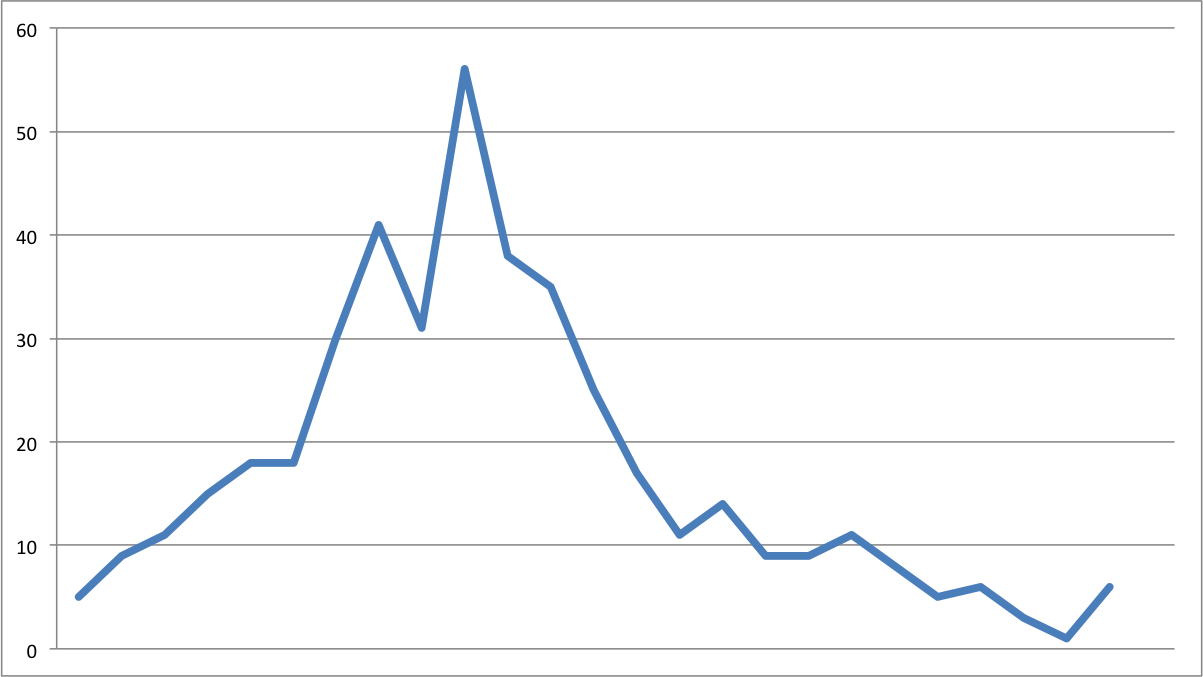
\includegraphics[width=4in]{../images/train_interarrivals/eastbound_blue_interarrivals.png}
\caption{\small \sl Eastbound Blue Line Interarrivals at Rosslyn. Ranges from 2.71 minutes to 16.78 with mean 10.91 \label{fig:eastboundblueinterarrivals}}
\end{center}
\end{figure}

\begin{figure}
\begin{center}
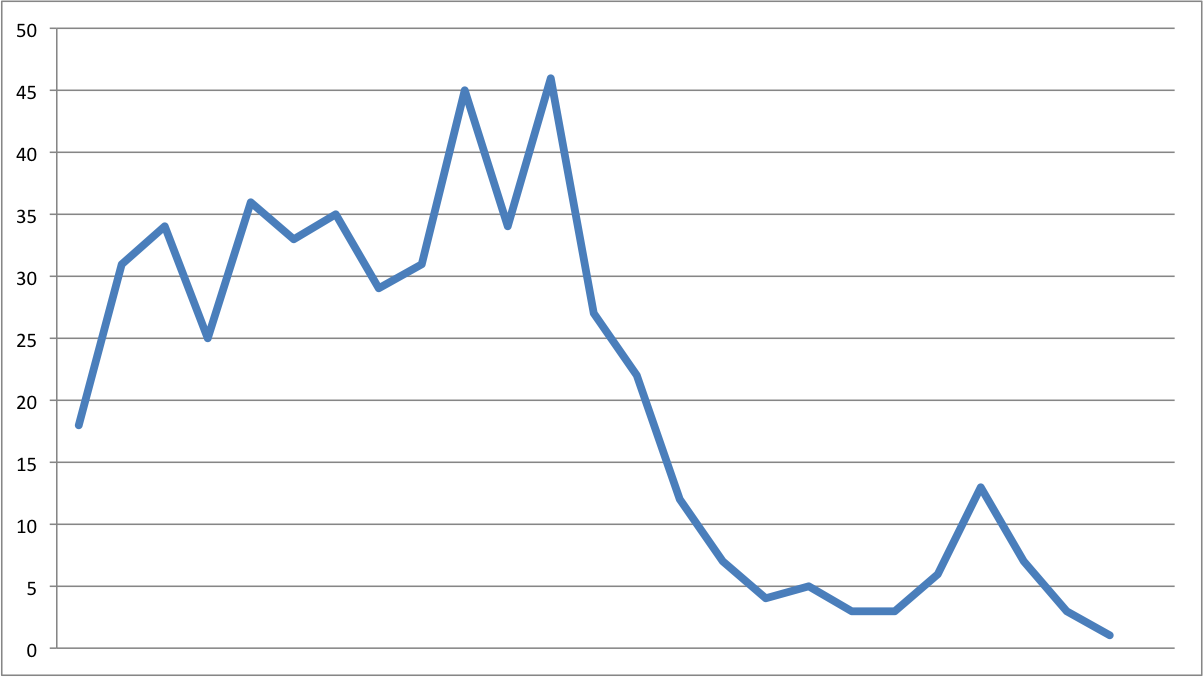
\includegraphics[width=4in]{../images/train_interarrivals/westbound_silver_interarrivals.png}
\caption{\small \sl Westbound Silver Line Interarrivals at Stadium Armory \label{fig:westboundsilverinterarrivals}}
\end{center}
\end{figure}


\section{Caveats and Limitations}

\section{Technology Used}

\section{Current and Remaining Work}

\bibliographystyle{plain}
\bibliography{main}

\end{document}
